\documentclass[a4paper]{report}

\usepackage[utf8]{inputenc}
\usepackage[T1]{fontenc}
\usepackage[american]{babel}
\usepackage{csquotes}
\usepackage[inline]{enumitem}
\usepackage{booktabs}
\usepackage[font=small,labelfont=bf]{caption}
\usepackage[group-separator={,}]{siunitx}
\usepackage{amsmath}
\usepackage{amssymb}
\usepackage{amsthm}
\usepackage{colonequals}
\usepackage{stmaryrd} % For double brackets \llbracket, \rrbracket
\usepackage[ruled,linesnumbered]{algorithm2e}
\usepackage{microtype}

\usepackage{listings}
\lstdefinestyle{mystyle}{
    basicstyle=\ttfamily\small\color{black!60},
    backgroundcolor=\color{black!5},
    commentstyle=\itshape\color{cyan},
    keywordstyle=\color{purple},
    keywordstyle=[2]\color{orange},
    identifierstyle=\color{black},
    numberstyle=\scriptsize\color{black},
    numbers=left,
    numbersep=4pt,
    columns=fixed,
}
\lstset{style=mystyle}
% Minimal support for WGSL, whatever is needed, based on C syntax
\lstdefinelanguage{WGSL}[ANSI]{C}%
    {morekeywords={let,var,fn},%
     morekeywords=[2]{u32,i32,bool},% Types
}

\usepackage{hyperref}
\hypersetup{
    colorlinks=true,
    linkcolor=blue,
    urlcolor=cyan,
    citecolor=teal,
    unicode=true,
}

\usepackage{tikz}
\usetikzlibrary{positioning,backgrounds}

\usepackage[style=numeric,urldate=ymd]{biblatex}
\addbibresource{bibliography.bib}

% Vertically centered vdots, taken from:
% https://tex.stackexchange.com/questions/112204/how-to-vertically-center-the-vdots-in-this-node
\makeatletter
\DeclareRobustCommand{\rvdots}{%
  \vbox{
    \baselineskip4\p@\lineskiplimit\z@
    \kern-\p@
    \hbox{.}\hbox{.}\hbox{.}
  }}
\makeatother

\theoremstyle{definition}
\newtheorem{definition}{Definition}

\newcommand{\upclosed}{\uparrow\!}

\begin{document}

\begin{titlepage}
    \centering

    \vspace*{4em}

    \LARGE
    \textbf{Accelerating Process Equivalence Energy Games using WebGPU}
    \vspace{2em}

    \large
    Bachelor's Thesis by

    Gabriel Vogel

    Matriculation No.: 413333
    \vspace{1em}

    \today
    \vspace{3em}

    \includegraphics{images/TU_Logo_kurz_RGB_rot.pdf}
    \vspace{3em}

    Technische Universität Berlin
    \vspace{5pt}

    Models and Theory of Distributed Systems
    \vfill

    \begin{tabular}{r@{: }l}
        Supervisor      &Benjamin Bisping \\
        First examiner  &Prof.~Dr.-Ing.~Uwe Nestmann \\
        Second examiner &Prof.~Dr.~Stephan Kreutzer \\
    \end{tabular}
    \vspace*{4em}
\end{titlepage}

%\begin{abstract}
%TODO Abstract
%\end{abstract}

\tableofcontents

\chapter{Introduction}
% Problem
In the field of process theory,
an often recurring question is that of
the behavioral similarity between processes in a transition system.
There are many different ways in which two processes can be considered
\emph{equivalent}.
In an important step towards grasping the range of equivalences,
\textcite{glabbeek1990spectrum} collected the most relevant definitions in the
so-called \emph{linear-time--branching-time spectrum}.
Being able to compute these equivalences is relevant for applications like
formal verification
or for gaining a better understanding of complex systems.

While algorithms for computing individual notions of equivalence
have long existed (e.g.~\cite{Blom2002}),
a process for deciding all equivalences of the spectrum at once
was only recently developed
by Bisping, Jansen and Nestmann~\cite{Bisping2022}.
This algorithm is subsequently refined by \textcite{bisping2023process}
where an \emph{energy game} is used for finding the equivalences.
This helps in bringing the runtime and memory usage of the algorithm down
to a more practical range,
but it is still very expensive to execute.
On larger inputs the implementation can easily run for the excess of several
minutes or even run out of memory.

% Contribution
This work aims to improve on that performance by utilizing the parallel
computing power of modern GPUs.
The idea is that large parts of the algorithm can be computed in parallel,
which, if successful, could result in a significant reduction in runtime.
To this end, the contribution of this thesis is the development
of \texttt{gpuequiv}%
\footnote{The code can be found at \url{https://github.com/Gobbel2000/gpuequiv}.
This document refers to version 1.0.0.},
a new, GPU-accelerated implementation
of the algorithm presented by \textcite{bisping2023process}.
It processes the most critical parts of the energy game in a highly
parallelized fashion
with the goal of making the spectroscopy algorithm faster and more scalable.
The same implementation can also be used more generally for solving energy
games.

For the task of interfacing with the GPU,
the WebGPU API is used.
WebGPU is a new web standard which currently is still in development,
with the goal of providing access to a system's GPU from web browsers.
By calling into WebGPU through the Rust library \texttt{wgpu} it is possible to
run the code both natively as well as from within a web site using WebAssembly.
This allows for very high platform-independence and portability.
Most of the code in \texttt{gpuequiv} is written in the
Rust programming language,
the GPU shaders are written in the WebGPU shading language WGSL\@.

\subsubsection{Related Work}

The broad structure for processing the energy game
is similar to a lot of other graph algorithms
by traversing the game graph in a breadth-first manner.
There is already a lot of research on running this category of graph
algorithms on a GPU~\cite{Merrill2015,Busato2018,Hijma2023}.
Similar projects exist in the context of transition systems,
for example a parallel algorithm for computing bisimilarity
by \textcite{Martens2023}
or a tool for detecting deadlocks in a transition system
by \textcite{Wijs2023},
both running on a GPU\@.
However, none of them give information
regarding the entire equivalence spectrum.

\subsubsection{Structure}

The following two chapters will introduce some of the concepts required to
fully understand the implementation choices behind \texttt{gpuequiv}.
Chapter~\ref{ch:processes} starts with defining processes and equivalences,
then continues to introducing the details of
the spectroscopy algorithm (\ref{sec:spectroscopy})
and of the energy game at its core (\ref{sec:energy_games}).
Chapter~\ref{ch:gpu} focuses on another important topic for this work:
GPU programming.
This includes details on the technology stack used
and the choice of WebGPU among other GPU frameworks,
followed by a short overview on what it means
to program for a GPU (\ref{sec:gpu_model}).

The actual GPU-based implementation of the spectroscopy algorithm is explained
in Chapter~\ref{ch:implementation}.
It begins with a more high-level look at how parallelization was achieved
(\ref{sec:parallelization}),
but also includes more technical details about the data layouts
used to efficiently handle the data (\ref{sec:data}).
Finally, in Chapter~\ref{ch:benchmarks} we will evaluate the performance
gained by parallelization with a series of benchmarks, which were
conducted both on \texttt{gpuequiv} as well as on the original implementation
by \textcite{bisping2023process}.


\chapter{Processes and Equivalences}
With the goal of introducing the algorithm for finding equivalences between
processes,
this chapter will introduce the theoretical concepts that this work is based on.
First and foremost this includes an explanation and definition
of the models we use to represent processes.
Further we will explore different ways to compare two processes and how that
leads us to the equivalence spectrum~\cite{glabbeek1990spectrum}.
Finally we will outline how the algorithm works,
that gives us a multifaceted view of the relation of two processes by testing
multiple of those equivalences at once~\cite{bisping2023process}.


\section{Modeling Processes}

We represent processes in a directed graph.
The outgoing edges of a node are the possible steps it can perform next.
Each edge is labelled with a specific action that occurs when taking that step.
After performing an action,
the process enters a new state represented by another node,
which is itself a process with its set of actions.
This forms a sort of state machine that at every step
moves to some other state by performing one of the currently available actions.
The series of actions being chosen
constitutes the observable behavior of the machine,
while its current state defines what actions it can do next.
Such a structure is called a \emph{Labeled transition system}
or \emph{LTS} for short~\cite{reactive_systems}.
Figure~\ref{fig:example_lts} gives an example for how the graph of an LTS might
look like.

\begin{definition}[Labeled transition system~\cite{reactive_systems}]
    A labeled transition system is a triple
    $(\mathsf{Proc}, \mathsf{Act}, {\rightarrow})$
    where:

    \begin{itemize}
        \item $\mathsf{Proc}$ is the set of states or processes,
        \item $\mathsf{Act}$ is a set of actions,
        \item ${\rightarrow} \subseteq \mathsf{Proc} \times \mathsf{Act} \times \mathsf{Proc}$
            is the transition relation.
            We also write
            $p \xrightarrow{\alpha} p'$ for $(p, \alpha, p') \in {\rightarrow}$,
            meaning we can transition from state $p$ to $p'$
            using the action $\alpha$.
    \end{itemize}
\end{definition}

\begin{figure}[htpb]
\begin{center}
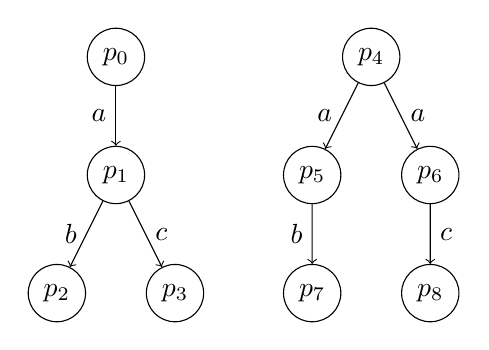
\begin{tikzpicture}[p/.style={circle,draw},->]
    \node[p] (0) {$p_0$}
        child {node[p] {$p_1$}
            child {node[p] {$p_2$} edge from parent node[left] {$b$}}
            child {node[p] {$p_3$} edge from parent node[right] {$c$}}
            edge from parent node[left] {$a$}
        };
    \node[p] (4) [right=25mm of 0] {$p_4$}
        child {node[p] {$p_5$}
            child {node[p] {$p_7$} edge from parent node[left] {$b$}}
            edge from parent node[left] {$a$}
        }
        child {node[p] {$p_6$}
            child {node[p] {$p_8$} edge from parent node[right] {$c$}}
            edge from parent node[right] {$a$}
        };
\end{tikzpicture}
\end{center}
\caption{An example for an LTS. In this case,
    $\mathsf{Proc} = \{p_0, p_1, \ldots, p_8\}$ and
    $\mathsf{Act} = \{a, b, c\}$.
}%
\label{fig:example_lts}
\end{figure}


\section{Equivalences between Processes}

% Trace Equivalence
% Bisimilarity
% Equivalences characterized by energies (through HML)


\section{Energy Games}\label{sec:energy_games}

\begin{definition}[Energy updates~\cite{bisping2023process}]\label{def:update}
    The set of $N$-dimensional energy updates $\mathbf{Up}_N$ contains
    $N$-tuples $(u_1, \ldots, u_N) \in \mathbf{Up}_N$ where each update $u_k, k
    \in [N]$ is
    either
    \begin{itemize}
        \item $u_k \in \{-1, 0\}$, or
        \item $u_k = \mathtt{min}_D$ where $D \subseteq [N]$ and $k \in D$. % chktex 35
    \end{itemize}

    The function
    $\mathsf{upd}_N: (\mathbf{En}_N, \mathbf{Up}_N) \rightarrow \mathbf{En}_N$
    applies an update to an energy tuple.
    The $k$-th component is given as:
    \begin{equation*}
        \mathsf{upd}_N{(e, u)}_k =
        \begin{cases}
            e_k + u_k,\quad &\text{if } u_k \in \{-1, 0\}, \\
            \min_{d \in D}{e_d},\quad &\text{if } u_k = \mathtt{min}_D. % chktex 35
        \end{cases}
    \end{equation*}
\end{definition}

\begin{definition}[Energy Games]\label{def:energy_game}
    We define an $N$-dimensional energy game as
    $(G, G_a, G_d, E, w, v_0)$, where 
    \begin{itemize}
        \item $G$ is a set of game positions.
        \item $G_a$ and $G_d$ are the sets of attacker and defender positions
            respectively.
            $G = G_a \cup G_d$ and $G_a \cap G_d = \emptyset$.
        \item $E \subseteq (G \times G)$ is the edge relation. $(G, E)$
            together form a directed game graph.
        \item $w: E \rightarrow \mathbf{Up}_N$ is a weight function, assigning an
            energy update to each edge.
        \item $v_0 \in G$ is the start position of the game.
    \end{itemize}

    The function $\mathrm{Succ}: G \rightarrow 2^G$ gives the successors in the
    graph for a position.
    For each $g \in G$, $\mathrm{Succ}(g) = \{g' \in G \mid (g, g') \in E\}$.
    Similarly, $\mathrm{Pred}(g) = \{g' \in G \mid (g', g) \in E\}$ yields a
    position's predecessors.
\end{definition}

\begin{definition}[Plays and costs]
    A \emph{play} $\rho$ on a given game is a sequence of positions:
    $\rho = g_0g_1 \ldots g_n$ where at each step
    $g_i \in G$ and $(g_i, g_{i+1}) \in E$.

    If a play cannot be further extended, that is,
    $\mathrm{Succ}(g_n) = \emptyset$,
    that play is won by the player who is not stuck:
    if $g_n \in G_a$, the defender wins, if $g_n \in G_d$, the attacker wins.
    Infinite plays are won by the defender.

    \scriptsize{TODO: costs}
\end{definition}

%TODO: Inverse update function upd^{-1}
%TODO: Energy tuples, upwards-closed sets, representation by minimal energies

\section{Spectroscopy Algorithm}



\chapter{GPU Compute Programming}\label{ch:gpu}
The core contribution of this work is a GPU-accelerated implementation of the
spectroscopy algorithm presented in~\cite{bisping2023process},
using the new WebGPU standard.
This chapter will give an overview on why WebGPU was chosen and how that
standard came to be among other GPU-compute frameworks.
Further we will discuss the GPU programming model,
how its massively parallelized architecture can be utilized
and which challenges it raises.

\section{WebGPU and the State of GPU-compute}

As their name suggests, Graphical Processing Units (GPUs) were initially built
to improve graphical processing capabilities of computer systems,
serving as \emph{graphics accelerators}.
At first they included mostly fixed-function hardware to run the usual
rendering pipeline.
This required the same calculations to be performed for every object to
be rendered and every pixel on the screen,
which was solved by running as much as possible in parallel in order to produce
fluent frame rates.
These graphics accelerators enabled real-time rendering performance far beyond
what is possible on a general-purpose CPU,
which is why their development was largely driven by the gaming industry.

But already early on people recognized the potential of using the parallel
GPU architecture not just for graphics rendering,
but for any kind of general-purpose computing that requires performing the same
instructions on a large amount of data.
GPUs gradually moved away from the fixed-function design and gained more
fine-grained programmability.
Along with that, specific programming environments were
developed to provide an easier interface for writing GPU compute programs.
Nvidia has long dominated the market by investing early in its
proprietary CUDA platform which supports Nvidia hardware only.
AMD has more recently been working on ROCm for their own GPUs.
OpenCL was meant to be a more portable alternative.

In another area WebGL was developed to bring GPU support into web browsers.
This was mainly intended for simpler graphics applications and is based on the
long-standing OpenGL graphics API\@.
Because of that, WebGL never really supported general-purpose compute programs.
Any efforts to improve this situation were abandoned%
\footnote{\url{https://registry.khronos.org/webgl/specs/latest/2.0-compute/}}
in favor of a new browser API\@: WebGPU\@.
Instead of OpenGL, WebGPU is based on more advanced graphics APIs
that expose modern GPU features:
Vulkan for Linux and Windows, DX12 for Windows and Metal for Apple.
General-purpose compute is one of the express features for WebGPU,
thus providing a GPU-programming API that is not only fully
platform-independent, but will even be able to run in any web browser.
However, as of the time of writing, the WebGPU specification is still in
development and full browser support is not yet available%
\footnote{\url{https://github.com/gpuweb/gpuweb/wiki/Implementation-Status}}.

For the GPU-code, this work uses \emph{wgpu}, an implementation of the WebGPU
standard written in the Rust programming language.
Applications using wgpu can both run natively, directly interfacing with the
operating system's graphics API,
or within a webpage through WebAssembly%
\footnote{WebAssembly is a sort of machine code format that many programming
languages, including Rust, can be compiled into
and then be executed by a web page.},
interfacing with the browser's WebGPU interface.
The Firefox browser even uses wgpu itself to implement WebGPU\@.


\section{Parallel Computing Model of a GPU}

\begin{figure}[ht]
\centering
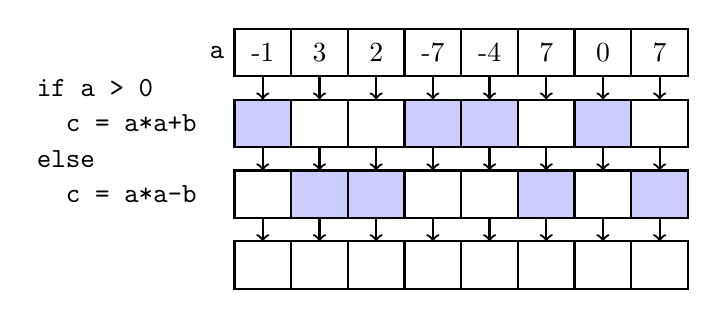
\begin{tikzpicture}[scale=0.6,thick]
    \foreach \x/\num in {0/-1, 1.2/3, 2.4/2, 3.6/-7, 4.8/-4, 6/7, 7.2/0, 8.4/7}
    {
        \draw (\x, 0) node {\num} +(-.6, -.5) rectangle ++(.6, .5);
        \ifnum \num > 0
            \draw (\x, -1.5) +(-.6, -.5) rectangle ++(.6, .5);
            \draw[fill=blue!20] (\x, -3) +(-.6, -.5) rectangle ++(.6, .5);
        \else
            \draw[fill=blue!20] (\x, -1.5) +(-.6, -.5) rectangle ++(.6, .5);
            \draw (\x, -3) +(-.6, -.5) rectangle ++(.6, .5);
        \fi
        \draw (\x, -4.5) +(-.6, -.5) rectangle ++(.6, .5);
        \draw[->] (\x, -0.5) -- (\x, -1);
        \draw[->] (\x, -2) -- (\x, -2.5);
        \draw[->] (\x, -3.5) -- (\x, -4);
    }
    \node[anchor=east] at (-0.6, 0)   {\verb|a|};
    \node[anchor=west] at (-5, -0.75) {\verb|if a > 0|};
    \node[anchor=west] at (-5, -1.5)  {\verb|  c = a*a+b|};
    \node[anchor=west] at (-5, -2.25) {\verb|else|};
    \node[anchor=west] at (-5, -3)    {\verb|  c = a*a-b|};
\end{tikzpicture}
\caption{Branch divergence in parallel execution.
    Shaded boxes indicate idle threads. Adapted from~\cite{Hijma2023}.
}\label{fig:branching}
\end{figure}


\chapter{Implementing the Spectroscopy Algorithm in WebGPU}\label{ch:implementation}
\section{Parallelizing the Algorithm}

At the center of this contribution is a parallel GPU-implementation%
\footnote{The code can be found at \url{https://github.com/Gobbel2000/gpuequiv}}
of the energy game introduced in section \ref{sec:energy_games}.
Given a game graph as input, it calcu\-lates for each position the energy budgets
required for the attacker, starting at the current position, to win the game.



\begin{figure}[h]
\begin{center}
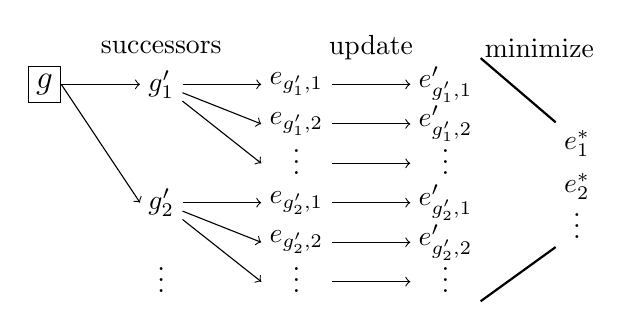
\begin{tikzpicture}[inner sep=1mm]
    \node[rectangle,draw] (start_node) {\large{$g$}};
    \node (successor1) [right=of start_node,label=above:successors] {$g_1'$};

    % Energies of successors
    \node (energy1_1) [right=of successor1] {$e_{g_1',1}$};
    \node (energy1_2) [below] at (energy1_1.south) {$e_{g_1',2}$};
    \node (dots1) [below] at (energy1_2.south) {\rvdots};
    \node (energy2_1) [below] at (dots1.south) {$e_{g_2',1}$};
    \node (energy2_2) [below] at (energy2_1.south) {$e_{g_2',2}$};
    \node (dots2) [below] at (energy2_2.south) {\rvdots};

    \node (successor2) [left=of energy2_1] {$g_2'$};
    \node (dots_successors) at (successor2 |- dots2) {\rvdots};

    % Updated energies
    \node (updated1_1) [right=of energy1_1] {$e_{g_1',1}'$};
    \node (updated1_2) [right=of energy1_2] {$e_{g_1',2}'$};
    \node (udots1) at (updated1_2 |- dots1) {\rvdots};
    \node (updated2_1) [right=of energy2_1] {$e_{g_2',1}'$};
    \node (updated2_2) [right=of energy2_2] {$e_{g_2',2}'$};
    \node (udots2) at (updated2_2 |- dots2) {\rvdots};
    % Include energies of g itself
    %\node (energyg_1) [below] at (udots2.south) {$e_{g,1}$};
    %\node (energyg_2) [below] at (energyg_1.south) {$e_{g,2}$};
    %\node (udots3) [below] at (energyg_2.south) {\rvdots};

    % Minimized energies
    \node (minimal1) [right=14mm of udots1.north] {$e_1^*$};
    \node (minimal2) [below] at (minimal1.south) {$e_2^*$};
    \node (mdots) [below] at (minimal2.south) {\rvdots};

    \draw[->] (start_node.east) -- (successor1.west);
    \draw[->] (start_node.east) -- (successor2.west);
    \draw[->] (successor1) -- (energy1_1.west);
    \draw[->] (successor1) -- (energy1_2.west);
    \draw[->] (successor1) -- (energy1_2.west |- dots1);
    \draw[->] (successor2) -- (energy2_1.west);
    \draw[->] (successor2) -- (energy2_2.west);
    \draw[->] (successor2) -- (energy2_2.west |- dots2);

    \draw[->] (energy1_1) -- node (l_update) [above=2mm] {update} (updated1_1);
    \draw[->] (energy1_2) -- (updated1_2);
    \draw[->] (energy1_2.east |- dots1) -- (updated1_2.west |- udots1);
    \draw[->] (energy2_1) -- (updated2_1);
    \draw[->] (energy2_2) -- (updated2_2);
    \draw[->] (energy2_2.east |- dots2) -- (updated2_2.west |- udots2);
    % Energies from g
    %\draw[->,shorten >= 4mm] (start_node.south) |-
    %    node [near end,below] {energies of $g$}
    %    (energyg_2.west);

    % Diagonal lines suggesting the reduction to minimal energies
    \draw[thick] (updated1_1.east |- udots2.south) -- (minimal1.west |- mdots.south);
    \draw[thick] (updated1_1.north east) -- (minimal1.north west);
    \node (l_minimize) [right=7mm of l_update] {minimize};
\end{tikzpicture}
\end{center}
\caption{Data flow for processing Attack positions}%
\label{fig:attack}
\end{figure}



\section{Data Layout}

\section{Control Flow}

\section{Limitations}


\chapter{Benchmarks and Evaluation of the Implementation}\label{ch:benchmarks}
This chapter will investigate the extent at which GPU-acceleration was able to
speed up execution of the spectroscopy algorithm.
Benchmarks were conducted to compare the performance of the new,
parallelized program \texttt{gpuequiv}
with the original implementation of the same algorithm by Bisping,
created alongside~\cite{bisping2023process}.
We will further look into what was done to verify the correctness of the GPU
implementation.

\section{Benchmarks}

The performance of the implementation was assessed by running it on files from
the \enquote{Very Large Transition System Benchmark Suite} (VLTS)~\cite{vlts},
which, as the name suggests,
includes transition systems with large numbers of states.
For the benchmark, the task is to find the equivalences between \emph{all}
process pairs within a transition system.
The energy game is constructed to include all process pairs that we want to
compare,
but there are some very impactful reductions we can apply to end up with
significantly less than $|\mathsf{Proc}|^2$ starting positions.

Firstly, we can minimize the LTS by consolidating bisimilar processes.
The bisimulation of an LTS can be computed quite efficiently---certainly much
faster than the full spectroscopy algorithm---with the help of a procedure
based around partition refinement~\cite{Blom2002}.
That way we end up with a smaller transition system with just one process for
each bisimulation class of the original system.
Because bisimilarity is already the strongest notion of equivalence,
all processes within a bisimulation class must behave the same for any
equivalence comparison,
so there is no information lost by performing this reduction step.

Secondly,
we can reduce the search space by inspecting the other end of the spectrum.
If two process already aren't enabledness-equivalent,
then none of the other equivalences can hold either,
making any further spectroscopy redundant.
Comparing the enabled actions of two processes is trivially easy,
so any starting positions comparing processes with distinct action sets
can simply be discarded.

\begin{table}[htpb]
    \centering
    \caption{Benchmarks}%
    \label{tab:benchmarks}
    \small
    \begin{tabular}{@{}l
                    r@{\hskip 6pt}r
                    r@{\hskip 6pt}r
                    S[table-format=3.3]@{}
                    S[table-format=3.4]@{\hskip 6pt}
                    S[table-format=1.4]@{}}
        \toprule
        &\multicolumn{2}{c}{LTS size}
        &\multicolumn{2}{c}{Game Graph size}
        &\multicolumn{3}{c}{Runtime (s)} \\
        \cmidrule(lr){2-3} \cmidrule(lr){4-5} \cmidrule(l){6-8}
        LTS~\cite{vlts}
        &$|\mathsf{Proc}|$ &$\sim_B$
        &$|G|$ &$|E|$
        &\cite{bisping2023process} &{gpuequiv} &{Game} \\
        \midrule

        \texttt{peterson}~\cite{bisping2023process}
                              &20     &19     &623        &1989        &0.137   &0.0058  &0.0054 \\
        \texttt{vasy\_0\_1}   &289    &9      &262        &788         &0.018   &0.0046  &0.0044 \\
        \texttt{vasy\_1\_4}   &1183   &28     &520        &1377        &0.019   &0.0052  &0.0050 \\
        \texttt{vasy\_5\_9}   &5486   &145    &1851       &3458        &0.039   &0.0056  &0.0050 \\
        \texttt{vasy\_8\_24}  &8879   &416    &59,551     &146,779     &1.347   &0.067   &0.042  \\
        \texttt{vasy\_8\_38}  &8921   &219    &7530       &20,575      &0.131   &0.0096  &0.0069 \\
        \texttt{vasy\_10\_56} &10,849 &2112   &1,949,100  &6,056,388   &109.027 &5.536   &4.068  \\
        \texttt{vasy\_18\_73} &18,746 &4087   &75,808,346 &623,498,702 &{--}    &112.083 &{--}   \\
        \texttt{vasy\_25\_25} &25,217 &25,217 &0          &0           &0.217   &0.0079  &0.0021 \\
        \texttt{cwi\_1\_2}    &1952   &1132   &8,503,473  &22,684,501  &228.989 &17.707  &9.283  \\
        \texttt{cwi\_3\_14}   &3996   &62     &11,094     &24,190      &0.192   &0.023   &0.019  \\
        \bottomrule
    \end{tabular}
\end{table}

\section{Correctness}


\chapter{Conclusion}
The idea of this work was to speed up the algorithm to find all equivalences
within a transition system~\cite{bisping2023process} by running it highly
parallelized on a GPU\@.
This objective was realized in the development of the open source software
library \texttt{gpuequiv}.
It can be used to find all equivalences notions of the
linear-time--branching-time spectrum~\cite{glabbeek1990spectrum}
that equate two or more processes.
This was accomplished with a GPU-accelerated algorithm for processing energy
games that can also be utilized for energy games in general,
not just in the context of the spectroscopy algorithm.
By building on the new WebGPU specification with the implementation of
\texttt{wgpu},
the code can not only run on all major platforms,
but even inside web browsers.

We have shown in Chapter~\ref{ch:implementation} how parallelization could be
applied to the spectroscopy algorithm.
It was found that large parts of work still had to be done on the CPU,
in particular when dealing with the dynamic graph data structures.
For example generation of the energy game graph had to be done full by the CPU
for these reasons.
The size of the game graph would have made it an enticing target for
optimization,
but in the end the time spent on generating the game by the CPU does not
outweigh the more complex solving of the resulting energy game.

The most critical parts of solving the energy game could successfully be
computed in parallel on the GPU\@.
This resulted in an overall significant uplift in performance compared to the
previous sequential implementation of~\cite{bisping2023process},
as shown by the benchmarks in Table~\ref{tab:benchmarks}:
The time required to process one particularly large transition system is
reduced from nearly 4 minutes down to just 18 seconds.

Even though care was taken to store data in a highly compressed format
(see~\ref{sec:data}),
the sheer size of the game graph needed to process larger inputs still
ended up exceeding memory limits.
It was therefore not possible to meaningfully increase scalability
over the original implementation.

\subsubsection{Further work}

While we have focused on the spectrum that was used
in~\cite{bisping2023process},
there is another version of the algorithm that includes many more equivalences
by accounting for silent steps~\cite{bisping2023silent}.
This requires a larger,
more complex game graph and energy values in 8 dimensions instead of 6.
Supporting these additional equivalences would be a way of expanding the
functionality of \texttt{gpuequiv}.
And there is of course always room for further optimization.


\printbibliography[heading=bibintoc]

\end{document}
